\section{Explanation of terms}

In this chapter we want to explain some of the phrases, words and terms used through out the article so the 
readers unfamiliar with version control might get an overall idea what version control is about.

\subsection{Repository}

A repository in DCVS terms is a folder which can contain sub folders and files of all categories. 
This folder is tracked by the DCVS so there is a history for every file whether it was renamed, deleted or changed. 
How these changes are tracked is different from system to system. CVS for example “isolates” 
files and handles them individually. So each file has its own version number. If you change a file, CVS will 
save the delta (i.e. what has changed) and give the file a new number. SVN does it a little bit 
different. If you change one file, the whole repository gets a new version number, usually count from 1, 2 to n. 
In SVN terms such a version of the repository is referred to as a “revision”.

Git also handles the repository as a whole. It saves each new file version as a whole and not just the delta as SVN and CVS does. 
In Git there are no incrementing version numbers, instead git uses the SHA-1 checksum. For each file there is such a 
checksum and the checksum which represents a certain revision is a sum of these checksums. 
This explanation might not be 100 percent correct but its a good approximation for those unfamiliar with version control.


\subsection{Commit}

Committing means that you make all your changes you have made to some files inside the repository permanent. 
After committing you have a new revision of your repository. Its possible to move back and forth between commits so you can work 
from an older version if you have screwed something up.

Normally with each commit there is saved some meta information like, who has committed and what has been done since the last commit. 
It's good practice to give detailed information about what files have changed and the purpose of these changes, so others working 
on the repository know whats going on.


\subsection{Checkout}

In CVS and SVN a checkout is the operation of creating a local working copy of a certain version from the 
central repository. In git checkout has a slightly different meaning. Creating a local working copy in git is 
called “clone”. Checkout is called the operation of switching between different versions and branches. I.e. 
you change your local working copy to another version.


\subsection{Branch}

Branching means that you diverge from your main line and continue working without messing up the main line of 
development. Branches are a feature where git really shines because they are very lightweight and really fast compared to other VCSs.

\begin{figure}[ht]
  \centering
  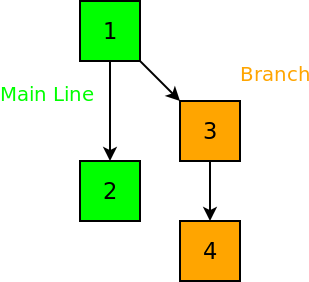
\includegraphics[width=0.4\textwidth]{img/Gen_Branch}
  \caption{Basic branching}
  \label{fig:gen_branch} 
\end{figure}

Figure \ref{fig:gen_branch} shows a little example how such a branch looks like. The green version 1 in 
this example is the initial commit with some files. Now developer A continues development in the main line 
by by fixing some bugs and improving the current version. Developer B know wants to add some new experimental 
features to version 1. Because developer B doesn't want to mess up the hopefully stable main line and the 
changes of developer A, he creates a branch where he can develop the new features until they are stable. 
So the orange versions 3 and 4 are the branch and the green versions is the stable main line.


\subsection{Merge}

Merging is called the process of integrating changes to a file which was modified by two people individually 
at the same time. When there are no conflicts the merge can be done automatically, else, a person must resolve 
the conflict. A conflict can occur when both people change the same lines inside a file, so the person who 
merges the changes must decide which version to use or how to integrate both versions into the file.

“Merging branches” does mean that changes made to a branch will be merged into another branch. 
To successfully merging branches they must have a common parent in their history.

\begin{figure}[ht]
  \centering
  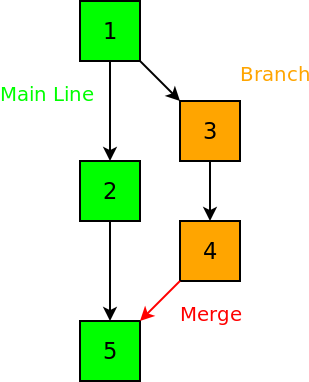
\includegraphics[width=0.4\textwidth]{img/Gen_Merge}
  \caption{Basic merging}
  \label{fig:gen_merge} 
\end{figure}

Figure \ref{fig:gen_merge} shows a later stage of the example from above. The developers decide that 
the new features in version 4 are stable and can be merged into the main line.


\subsection{Tagging}

Tagging means that you mark a certain version or revision with a tag. 
Assigning a tag to a version is just for convenience, normally its used to tag important project milestones. 
For example if your application which you are developing reaches version 1.5, you will assign a tag named “v1.5” 
to the commit or revision which was used to build the “application 1.5” or which represents the “application 1.5”. 
So it will be very easy to find the commit you need in the future if you want an older version of your application.

\begin{figure}[ht]
  \centering
  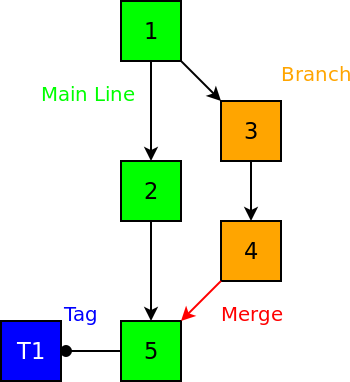
\includegraphics[width=0.4\textwidth]{img/Gen_Tag}
  \caption{Basic tagging}
  \label{fig:gen_tag}
\end{figure}

Figure \ref{fig:gen_tag} shows how the new version 5 from above is tagged with a tag T1.
